\documentclass[journal,12pt,onecolumn]{IEEEtran}
\usepackage{cite}
\usepackage{graphicx}
\usepackage{amsmath,amssymb,amsfonts,amsthm}
\usepackage{algorithmic}
\usepackage{graphicx}
\usepackage{textcomp}
\usepackage{xcolor}
\usepackage{txfonts}
\usepackage{listings}
\usepackage{enumitem}
\usepackage{mathtools}
\usepackage{gensymb}
\usepackage{comment}
\usepackage[breaklinks=true]{hyperref}
\usepackage{tkz-euclide} 
\usepackage{listings}
\usepackage{gvv}                                        
%\def\inputGnumericTable{}                                 
\usepackage[latin1]{inputenc} 
\usetikzlibrary{arrows.meta, positioning}
\usepackage{xparse}
\usepackage{color}                                            
\usepackage{array}                                            
\usepackage{longtable}                                       
\usepackage{calc}                                             
\usepackage{multirow}
\usepackage{multicol}
\usepackage{hhline}                                           
\usepackage{ifthen}                                           
\usepackage{lscape}
\usepackage{tabularx}
\usepackage{array}
\usepackage{float}
\newtheorem{theorem}{Theorem}[section]
\newtheorem{problem}{Problem}
\newtheorem{proposition}{Proposition}[section]
\newtheorem{lemma}{Lemma}[section]
\newtheorem{corollary}[theorem]{Corollary}
\newtheorem{example}{Example}[section]
\newtheorem{definition}[problem]{Definition}
\newcommand{\BEQA}{\begin{eqnarray}}
\newcommand{\EEQA}{\end{eqnarray}}
\usepackage{float}
%\newcommand{\define}{\stackrel{\triangle}{=}}
\theoremstyle{remark}
\usepackage{circuitikz}
\usepackage{tikz}

\title{IN  INSTRUMENTATION ENGINEERING}
\author{EE25BTECH11031- Sai Sreevallabh}

\author{Sai Sreevallabh - ee25btech11031}

\begin{document}

\maketitle

\section*{\underline{General Aptitude (GA)}}

\textbf{Q.1-Q.5 Multiple Choice Question(MCQ), carry ONE mark each (for wrong answer, -1/3)}

\begin{enumerate}
%1 
\item Getting to the top is \rule{1.5cm}{0.4pt} than staying on top
\par \hfill\brak{\text{GATE IN 2021}}
\begin{enumerate}
    \begin{multicols}{4}
        \item more easy
        \item much easy
        \item easier
        \item easiest
    \end{multicols}
\end{enumerate}

\item \begin{figure}[H]
    \centering
    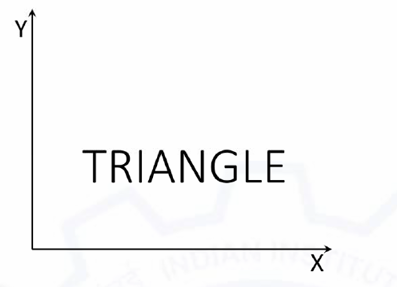
\includegraphics[width=0.5\linewidth]{Figs/Q-2(GA).png}
    \caption{Image for Question-2}
    \label{2}
\end{figure} 
The mirror image of the above text (\figref{2}) is about the x-axis is \par \hfill\brak{\text{GATE IN 2021}}
\begin{enumerate}
    \item . \begin{figure}[H]
    \centering
    
\includegraphics[width=0.15\linewidth]{Figs/Q-2(option1)(GA).png}
    \end{figure}
        
    \item . \begin{figure}[H]
    \centering
    
\includegraphics[width=0.15\linewidth]{Figs/Q-2(optionB)(GA).png}
    \end{figure} 
    
    \item . \begin{figure}[H]
    \centering
    
\includegraphics[width=0.15\linewidth]{Figs/Q-2(optionC)(GA).png}
    \end{figure} 
    
    \item . \begin{figure}[H]
    \centering
    
\includegraphics[width=0.15\linewidth]{Figs/Q-2(optionD)(GA).png}
    \end{figure} 
\end{enumerate}

%3
\item In a company, $35\%$ of the employees drink coffee, $40\%$ of the employees drink tea and $10\%$ of the employees drink both tea and coffee. What \% of employees drink neither tea nor coffee?\par \hfill\brak{\text{GATE IN 2021}}
\begin{enumerate}
\begin{multicols}{4}
  \item $15$
  \item $25$
  \item $35$
  \item $40$
\end{multicols}
\end{enumerate}

%4
\item $\oplus$ and $\odot$ are two operators on numbers $p$ and $q$ such that
$$p{\oplus}q= \frac{p^2+q^2 }{pq}$$ 
and $$p{\odot}q = \frac{p^2}{q}$$; If $x{\oplus}y = 2\odot{2}$, then $x=$
\par \hfill\brak{\text{GATE IN 2021}}
\begin{enumerate}
\begin{multicols}{4}
  \item $y/2$
  \item $y$
  \item $3y/2$
  \item $2y$
\end{multicols}
\end{enumerate}

%5
\item Four persons P, Q, R and S are to be seated in a row, all facing the same direction, but not necessarily in the same order. P and R cannot sit adjacent to each other. S should be seated to the right of Q. The number of distinct seating arrangements possible is
\par \hfill\brak{\text{GATE IN 2021}}
\begin{enumerate}
\begin{multicols}{4}
  \item $2$
  \item $4$
  \item $6$
  \item $8$
\end{multicols}
\end{enumerate}

\textbf{Q.6 -- Q.10 : Multiple Choice Question(MCQ), Carry TWO marks each (For each wrong answer: ${2/}{3}$)}

% -------- Q6 ----------
\item Statement: Either P marries Q or X marries Y.  
Among the options below, the logical NEGATION of the above statement is
\par \hfill\brak{\text{GATE IN 2021}}
\begin{enumerate}
  \item P does not marry Q and X marries Y.
  \item Neither P marries Q nor X marries Y.
  \item X does not marry Y and P marries Q.
  \item P marries Q and X marries Y.
\end{enumerate}

% -------- Q7 ----------
\item Consider two rectangular sheets, Sheet M and Sheet N of dimensions $6 cm \times 4 cm$ each.  
Folding operation 1: The sheet is folded into half by joining the short edges of the current shape.  
Folding operation 2: The sheet is folded into half by joining the long edges of the current shape.  
Folding operation 1 is carried out on Sheet M three times.  
Folding operation 2 is carried out on Sheet N three times.  
The ratio of perimeters of the final folded shape of Sheet N to the final folded shape of Sheet M is
\par \hfill\brak{\text{GATE IN 2021}}
\begin{enumerate}
\begin{multicols}{4}
  \item $13:7$
  \item $3:2$
  \item $7:5$
  \item $5:13$
\end{multicols}
\end{enumerate}

% -------- Q8 ----------
\item % Figure placeholder for star diagram
Five line segments of equal lengths, PR, PS, QS, QT and RT are used to form a star as shown in \figref{8(GA)}.  
The value of $\theta$, in degrees, is
\begin{figure}[H]
    \centering
    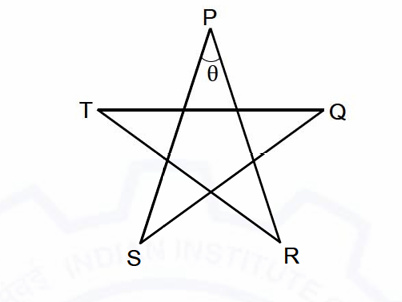
\includegraphics[width=0.4\linewidth]{Figs/Q-8(GA).png}
    \caption{Star}
    \label{8(GA)}
\end{figure}
\par \hfill\brak{\text{GATE IN 2021}}
\begin{enumerate}
\begin{multicols}{4}
  \item $36$
  \item $45$
  \item $72$
  \item $108$
\end{multicols}
\end{enumerate}

% -------- Q9 ----------
\item A function, $\lambda$, is defined by
$$\lambda(p,q) =
\begin{cases}
 \brak{p-q}^2, & p\ge q \\
 p+q, & p<q
\end{cases}$$

The value of the expression
$$\frac{ \lambda\brak{-\brak{-3+2},\brak{-2+3}}}{ -\brak{-2+1} }$$
is \par \hfill\brak{\text{GATE IN 2021}}
\begin{enumerate}
\begin{multicols}{4}
  \item $-1$
  \item $0$
  \item $16/3$
  \item $16$
\end{multicols}
\end{enumerate}

% -------- Q10 ----------
\item Humans have the ability to construct worlds entirely in their minds, which don't exist in the physical world. So far as we know, no other species possesses this ability. This skill is so important that we have different words to refer to its different flavors, such as imagination, invention and innovation.  

Based on the above passage, which one of the following is TRUE?
\par \hfill\brak{\text{GATE IN 2021}}
\begin{enumerate}
  \item No species possess the ability to construct worlds in their minds.
  \item The terms imagination, invention and innovation refer to unrelated skills.
  \item We do not know of any species other than humans who possess the ability to construct mental worlds.
  \item Imagination, invention and innovation are unrelated to the ability to construct mental worlds.
\end{enumerate}

\end{enumerate}

\section*{\textbf{\underline{Instrumentation Engineering (IN)}}}

\textbf{Q.1 -- Q.8 : MCQ, 1 mark each (Negative marks: $-1/3$)}

\begin{enumerate}
\item Consider the row vectors $v =\brak{1,0}$ and $w =\brak{2,0}$. The rank of the matrix $M = 2v^Tv + 3w^T w$, where the superscript $T$ denotes the transpose, is \par \hfill\brak{\text{GATE IN 2021}}
\begin{enumerate}
\begin{multicols}{4}
  \item $1$
  \item $2$
  \item $3$
  \item $4$
\end{multicols}
\end{enumerate}

\item Consider the sequence $x_n = 0.5x_{n-1}+1, \; n = 1, 2, \dots$ with $x_0=0$. Then  
$\lim\limits_{n\to\infty} x_n$ is \par \hfill\brak{\text{GATE IN 2021}}
\begin{enumerate}
\begin{multicols}{4}
  \item $0$
  \item $1$
  \item $2$
  \item $\infty$
\end{multicols}
\end{enumerate}

% Q.3
\item An infinitely long line, with uniform positive charge density, lies along the $z$-axis. In cylindrical coordinates $(r, \phi, z)$, at any point $\Vec{P}$ not on the $z$-axis, the direction of the electric field is \par \hfill\brak{\text{GATE IN 2021}}
\begin{enumerate}
\begin{multicols}{4}
\item $\hat{\text{r}}$
\item $\hat{{\phi}}$
\item $\hat{{z}}$
\item $\frac{\brak{\hat{r}+\hat{z}}}{\sqrt{2}}$
\end{multicols}
\end{enumerate}

% Q.4
\item The input-output relationship of an LTI system is given below (\figref{4(1)})
\begin{figure}[H]
    \centering
    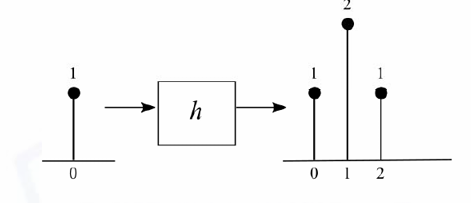
\includegraphics[width=0.5\linewidth]{Figs/Q-4(fig-1).png}
    \caption{Input Output relationship of an LTI System}
    \label{4(1)}
\end{figure}
For an input $x\sbrak{n}$ shown below (\figref{4(2)})
\begin{figure}[H]
    \centering
    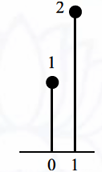
\includegraphics[width=0.1\linewidth]{Figs/Q-4(fig-2).png}
    \caption{Input}
    \label{4(2)}
\end{figure}
the peak value of the output when $x\sbrak{n}$ passes through $h$ is \par \hfill\brak{\text{GATE IN 2021}}
\begin{enumerate}
\begin{multicols}{4}
\item $2$
\item $4$
\item $5$
\item $6$
\end{multicols}
\end{enumerate}

% Q.5
\item In an AC main, the RMS voltage $V_{\mathrm{ac}}$, RMS current $I_{\mathrm{ac}}$ and power $W_{\mathrm{ac}}$ are measured as: $V_{\mathrm{ac}} = 100\,\mathrm{V} \pm 1\%$, $I_{\mathrm{ac}} = 1\,\mathrm{A} \pm 1\%$ and $W_{\mathrm{ac}} = 50\,\mathrm{W} \pm 2\%$ (errors are with respect to readings). The percentage error in calculating the power factor using these readings is \par \hfill\brak{\text{GATE IN 2021}}
\begin{enumerate}
\begin{multicols}{4}
\item $1\%$
\item $2\%$
\item $3\%$
\item $4\%$
\end{multicols}
\end{enumerate}

% Q.6
\item Let $u\brak{t}$ denote the unit step function. The bilateral Laplace transform of the function $f\brak{t} = e^t u\brak{-t}$ is \par \hfill\brak{\text{GATE IN 2021}}
\begin{enumerate}
\begin{multicols}{2}
\item $\frac{1}{s-1}$ with real part of $s < 1$
\item $\frac{1}{s-1}$ with real part of $s > 1$
\item $\frac{-1}{s-1}$ with real part of $s < 1$
\item $\frac{-1}{s-1}$ with real part of $s > 1$
\end{multicols}
\end{enumerate}


% Q.7
\item Input-output characteristic of a temperature sensor is exponential for a \par \hfill\brak{\text{GATE IN 2021}}
\begin{enumerate}
\begin{multicols}{2}
\item Thermistor
\item Thermocouple
\item Resistive Temperature Device (RTD)
\item Mercury thermometer
\end{multicols}
\end{enumerate}

% Q.8
\item The signal $\sin(\sqrt{2}\pi t)$ is \par \hfill\brak{\text{GATE IN 2021}}
\begin{enumerate}
\begin{multicols}{2}
\item periodic with period $T = \sqrt{2\pi}$
\item not periodic
\item periodic with period $T = 2\pi$
\item periodic with period $T = 4\pi^2$
\end{multicols}
\end{enumerate}

%%%%%%%%%%%%%SOME INSTRUCTIONS%%%%%%%%%%%%%%%%%

% Q.9
\item The step response of a circuit is seen to have an oscillatory behaviour at the output with oscillations dying down after some time. The correct inference(s) regarding the transfer function from input to output is/are \par \hfill\brak{\text{GATE IN 2021}}
\begin{enumerate}
\item that it is of at least second order.
\item that it has at least one pole-pair that is underdamped.
\item that it does not have a real pole.
\item that it is a first-order system.
\end{enumerate}

% Q.10
\item For a $4$-bit Flash type Analog to Digital Converter (ADC) with full-scale input voltage range ``$V$'', which of the following statement(s) is/are true? \par \hfill\brak{\text{GATE IN 2021}}
\begin{enumerate}
\item The ADC requires $15$ comparators.
\item The ADC requires one $4$ to $2$ priority encoder and $4$ comparators.
\item A change in the input voltage by $\frac{V}{16}$ will always flip MSB of the output.
\item A change in the input voltage by $\frac{V}{16}$ will always flip LSB of the output.
\end{enumerate}

% Q.11
\item A $16$-bit microprocessor has twenty address lines ($A_0$ to $A_{19}$) and $16$ data lines. The higher eight significant lines of the data bus of the processor are tied to the 8-data lines of a $16$ Kbyte memory that can store one byte in each of its $16$K address locations. The memory chip should map onto contiguous memory locations and occupy only $16$ Kbyte of memory space. Which of the following statement(s) is/are correct with respect to the above design? \par \hfill\brak{\text{GATE IN 2021}}
\begin{enumerate}
\item If the $16$Kbyte of memory chip is mapped with a starting address of $80000$H, then the ending address will be $83$FFFH.
\item The active high chip-select needed to map the $16$Kbyte memory with a starting address at F$0000$H is given by the logic expression $(A_{19} \cdot A_{18} \cdot A_{17} \cdot A_{16})$.
\item The $16$Kbyte memory cannot be mapped with contiguous address locations with a starting address as $0$F$000$H using only $A_{19}$ to $A_{14}$ for generating chip-select.
\item The above chip cannot be interfaced as the width of the data bus of the processor and the memory chip differs.
\end{enumerate}

% Q.12
\item A single-phase transformer has a magnetizing inductance of $250\ \text{mH}$ and a core loss resistance of $300\ohm$, referred to primary side. When excited with a $230\text{V}$, $50\text{Hz}$ sinusoidal supply at the primary, the power factor of the input current drawn, with secondary on open circuit, is\rule{1cm}{0.4pt} (rounded off to two decimal places).  \par \hfill\brak{\text{GATE IN 2021}} 

% Q.13
\item Taking $N$ as positive for clockwise encirclement, otherwise negative, the number of encirclements $N$ of $\brak{-1,0}$ in the Nyquist plot of $G\brak{s} = \frac{3}{s-1}$ is \rule{1.5cm}{0.4pt}   \par \hfill\brak{\text{GATE IN 2021}}


% Q.14
\item The diode used in the circuit has a fixed voltage drop of $0.6\ \text{V}$ when forward biased. A signal $v_s$ is given to the ideal OpAmp as shown in \figref{14} When $v_s$ is at its positive peak, the output $V_{\text{OA}}$ of the OpAmp in volts is \rule{1.5cm}{0.4pt}. \par \hfill\brak{\text{GATE IN 2021}}
\begin{figure}[H]
    \centering
    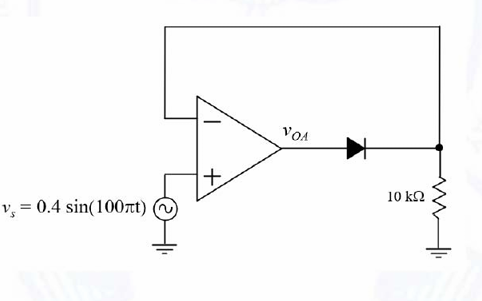
\includegraphics[width=0.5\linewidth]{Figs/Q-14.png}
    \caption{Circuit Diagram for Question-14}
    \label{14}
\end{figure}

% Q.15
\item The transistor $Q_1$ (in \figref{15)} has a current gain $\beta_1 = 99$ and the transistor $Q_2$ has a current gain $\beta_2 = 49$. The current $I_{B2}$ in microampere is \rule{1.5cm}{0.4pt}  \par \hfill\brak{\text{GATE IN 2021}}
\begin{figure}[H]
    \centering
    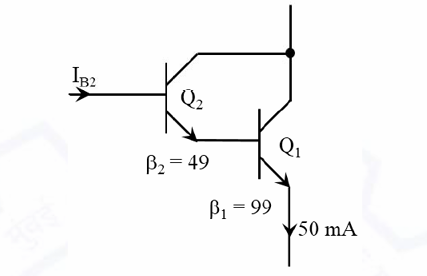
\includegraphics[width=0.5\linewidth]{Figs/Q-15.png}
    \caption{Circuit Diagram for Question-15}
    \label{15}
\end{figure}


% Q.16
\item A $300\ \text{V}$, $5\ \text{A}$, LPF wattmeter has a full scale of $300\ \text{W}$. 
The wattmeter can be used for loads supplied by $300\ \text{V}$ AC mains with a maximum power factor of 
\rule{1.5cm}{0.4pt} (rounded off to one decimal place). \par \hfill\brak{\text{GATE IN 2021}}

% Q.17
\item A $10$-bit ADC has a full-scale of $10.230\ \text{V}$, when the digital output is $11\ 1111\ 1111_2$. 
The quantization error of the ADC in millivolt is \rule{1.5cm}{0.4pt}. \par \hfill\brak{\text{GATE IN 2021}}

% Q.18
\item A strain gage having nominal resistance of $1000\ \ohm$ has a gage factor of $2.5$. 
If the strain applied to the gage is $100\ \mu m/m$, its resistance in ohm will change to 
\rule{1.5cm}{0.4pt} (rounded off to two decimal places) \par \hfill\brak{\text{GATE IN 2021}}

% Q.19
\item Given: Density of mercury is $13600\ \text{kg/m}^3$ and $g=9.81\ \text{m/s}^2$. 
Atmospheric pressure is $101\ \text{kPa}$. In a mercury U-tube manometer, the difference between the heights of the liquid in the U-tube is $1\ \text{cm}$. 
The differential pressure being measured in Pascal is \rule{1.5cm}{0.4pt} (rounded off to the nearest integer). \par \hfill\brak{\text{GATE IN 2021}}

% Q.20
\item A piezoresistive pressure sensor has a sensitivity of $1\ \brak{\text{mV/V}}/\text{kPa}$. 
The sensor is excited with a DC supply of $10\ \text{V}$ and the output is read using a $3\frac{1}{2}$ digit $200\ \text{mV}$ full-scale DMM. 
The resolution of the measurement set-up, in Pascal is \rule{1.5cm}{0.4pt}. \par \hfill\brak{\text{GATE IN 2021}}

% Q.21
\item An amplitude modulation (AM) scheme uses tone modulation, with modulation index $0.6$. 
The power efficiency of the AM scheme is \rule{1.5cm}{0.4pt} \% (rounded off to one decimal place). \par \hfill\brak{\text{GATE IN 2021}}

% Q.22
\item When the movable arm of a Michelson interferometer in vacuum $\brak{n=1}$ is moved by $325\mu m$, the number of fringe crossings is $1000$. The wavelength of the laser used in nanometers is \rule{1.5cm}{0.4pt}. \par \hfill\brak{\text{GATE IN 2021}}

% Q.23
\item Consider $f\brak{x} = -x^2 + 10x + 100$. The minimum value of the function in the interval $\sbrak{5, 10}$ is \rule{1.5cm}{0.4pt}. \par \hfill\brak{\text{GATE IN 2021}}

% Q.24
\item Let $f\brak{z} = \frac{1}{z^2+6z+9}$ defined in the complex plane. 
The integral $\oint_c f\brak{z}dz$ over the contour of a circle $c$ with center at the origin and unit radius is \rule{1.5cm}{0.4pt}. \par \hfill\brak{\text{GATE IN 2021}}

% Q.25
\item The determinant of the matrix $\textbf{M}$ shown below is \rule{1.5cm}{0.4pt}. \par \hfill\brak{\text{GATE IN 2021}}
$$M = \myvec{
1 & 2 & 0 & 0 \\
3 & 4 & 0 & 0 \\
0 & 0 & 4 & 3 \\
0 & 0 & 2 & 1
}$$


% Q.26
\item $f\brak{z} = \brak{z-1}^{-1} - 1 + \brak{z-1} - \brak{z-1}^2 + \ldots$ is the series expansion of   \par \hfill\brak{\text{GATE IN 2021}}
\begin{enumerate}[label=(\Alph*)]
\begin{multicols}{2}
\item $\dfrac{-1}{z\brak{z-1}}$ for ${|z-1|<1}$
\item $\dfrac{1}{z\brak{z-1}}$ for ${|z-1|<1}$
\item $\dfrac{1}{\brak{z-1}^2}$ for ${|z-1|<1}$
\item $\dfrac{-1}{z-1}$ for ${|z-1|<1}$
\end{multicols}
\end{enumerate}

% Q.27
\item A single-phase transformer has maximum efficiency of $98 \%$. The core losses
are $80\ \text{W}$ and the equivalent winding resistance as seen from the primary
side is $0.5\ \ohm$. The rated current on the primary side is $25\ \text{A}$. The percentage
of the rated input current at which the maximum efficiency occurs is \par \hfill\brak{\text{GATE IN 2021}}
\begin{enumerate}[label=(\Alph*)]
\begin{multicols}{4}
\item $35.7\%$
\item $50.6\%$
\item $80.5\%$
\item $100\%$
\end{multicols}
\end{enumerate}

% Q.28
\item A slip-ring induction motor is expected to be started by adding extra
resistance in the rotor circuit. The benefit that is derived by adding extra
resistance in the rotor circuit in comparison to the rotor being shorted is \par \hfill\brak{\text{GATE IN 2021}}
\begin{enumerate}[label=(\Alph*)]
\item The starting torque would be higher.
\item The power factor at start will be lower.
\item The starting current is higher.
\item The losses at starting would be lower.
\end{enumerate}

% Q.29
\item Consider a unity feedback configuration with a plant and a PID controller as shown in \figref{29}. $G\brak{s} = \frac{1}{\brak{s+1}\brak{s+3}}$
and $C\brak{s} = K\frac{\brak{s+3-j}\brak{s+3+j}}{s}$
with $K$ being scalar. The closed loop is \par \hfill\brak{\text{GATE IN 2021}}
\begin{figure}[H]
    \centering
    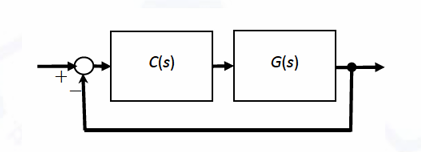
\includegraphics[width=0.5\linewidth]{Figs/Q-29.png}
    \caption{Unity Feedback Configuration}
    \label{29}
\end{figure}
\begin{enumerate}[label=(\Alph*)]
\begin{multicols}{2}
\item only stable for $K > 0$
\item only stable for $K$ between $-1$ and $+1$
\item only stable for $K < 0$
\item stable for all values of $K$
\end{multicols}
\end{enumerate}

% Q.30
\item The output $V_o$ of the ideal OpAmp used in the circuit shown in \figref{30} is $5\ \text{V}$.
The value of resistor $\text{R}_\text{L}$ in kilo ohm ($\text{k}\ohm$) is \par \hfill\brak{\text{GATE IN 2021}}
\begin{figure}[H]
    \centering
    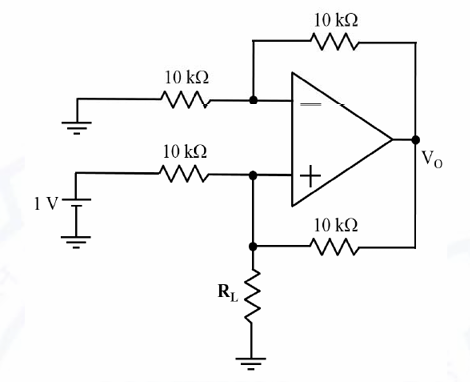
\includegraphics[width=0.5\linewidth]{Figs/Q-30.png}
    \caption{Circuit Diagram for Question-30}
    \label{30}
\end{figure}
\begin{enumerate}[label=(\Alph*)]
\begin{multicols}{4}
\item $2.5$
\item $5$
\item $25$
\item $50$
\end{multicols}
\end{enumerate}

% Q.31
\item A Boolean function $F$ of three variables $X,\ Y,\ \text{and}\ Z$ is given as  
\[F\brak{X, Y, Z} = \brak{X' + Y + Z}\cdot\brak{X + Y' + Z'}\cdot\brak{X' + Y + Z'}\cdot
\brak{X'Y'Z' + X'YZ' + XYZ'}\]  
Which one of the following is true? \par \hfill\brak{\text{GATE IN 2021}}
\begin{enumerate}[label=(\Alph*)]
\begin{multicols}{2}
\item $F\brak{X,Y,Z} = \brak{X + Y + Z'}\cdot\brak{X' + Y' + Z'}$
\item $F\brak{X,Y,Z} = \brak{X' + Y}\cdot\brak{X + Y + Z'}$
\item $F\brak{X,Y,Z} = X'Z' + YZ'$
\item $F\brak{X,Y,Z} = X'Y'Z + XYZ$
\end{multicols}
\end{enumerate}

% Q.32
\item A $10\frac{1}{2}$ digit Counter-timer is set in the 'frequency mode' of operation (with $T_s = 1\ \text{s}$). For a specific input, the reading obtained is $1000$. Without disconnecting this input, the Counter-timer is changed to operate in the 'Period mode' and the range selected is microseconds ($\mu \text{s}$, with $f_s = 1\ \text{MHz}$).
The counter will then display \par \hfill\brak{\text{GATE IN 2021}}
\begin{enumerate}[label=(\Alph*)]
\begin{multicols}{4}
\item $0$
\item $10$
\item $100$
\item $1000$
\end{multicols}
\end{enumerate}

% Q.33
\item A J-type thermocouple has an output voltage $V_o = \brak{13650 + 50\ \theta x}\ \mu\text{V}$, where $\theta x$ is the junction temperature in Celsius ($^\circ \text{C}$). The thermocouple is used with
reference junction compensation, as shown in \figref{33}. The
Instrumentation amplifier used has a gain $G = 20$. If $\theta_{\text{ref}}$ is $1^\degree \text{C}$, for an input
$\theta x$ of $100^\degree \text{C}$, the output $V_o$ of the instrumentation amplifier in millivolt is 
\begin{figure}[H]
    \centering
    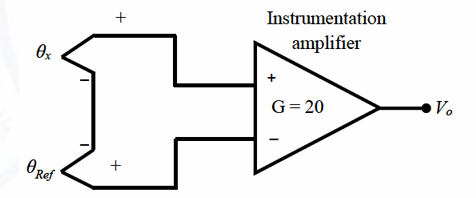
\includegraphics[width=0.5\linewidth]{Figs/Q-33.png}
    \caption{J-Type Thermocouple}
    \label{33}
\end{figure}
\par \hfill\brak{\text{GATE IN 2021}}
\begin{enumerate}[label=(\Alph*)]
\begin{multicols}{4}
\item $98\ \text{mV}$
\item $99\ \text{mV}$
\item $100\ \text{mV}$
\item $101\ \text{mV}$
\end{multicols}
\end{enumerate}

% Q.34
\item A laser pulse is sent from ground level to the bottom of a concrete water tank at normal incidence as in \figref{34}. The tank is filled with water up to $2\ \text{m}$ below the ground level. The reflected pulse from the bottom of the tank travels back and hits the detector. The round-trip time elapsed between sending the laser pulse, the pulse hitting the bottom of the tank, reflecting back and sensed by the  etector is $100\ \text{ns}$. The depth of the tank from ground level marked as $x$ in
metre is \rule{1.5cm}{0.4pt} (Refractive index of water $n_{water}=1.3$ and velocity of light in air $c_{air} = 3 \times 10^8\ \text{m/s}$) \par \hfill\brak{\text{GATE IN 2021}}
\begin{figure}[H]
    \centering
    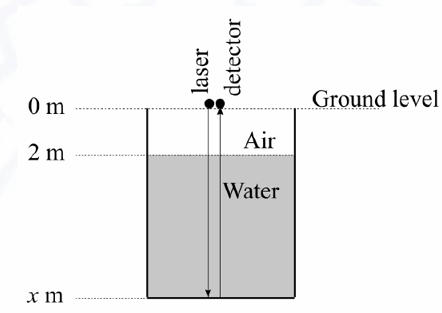
\includegraphics[width=0.5\linewidth]{Figs/Q-34.png}
    \caption{Incidence of Laser into the Water}
    \label{34}
\end{figure}
\begin{enumerate}[label=(\Alph*)]
\begin{multicols}{4}
\item $9$
\item $10$
\item $11$
\item $12$
\end{multicols}
\end{enumerate}

% Q.35
\item A $4 \times 1$ multiplexer with two selector lines is used to realize a Boolean function $F$ having four Boolean variables $X, Y, Z \text{and} W$ as shown in \figref{35}. So $S_0$ and $S_1$ denote the least significant bit (LSB) and most significant bit (MSB) of the selector lines of the multiplexer respectively. $I_0, I_1, I_2, I_3$ are the input lines of the multiplexer. The canonical sum of product representation of $F$ is \par \hfill\brak{\text{GATE IN 2021}}

\begin{figure}[H]
    \centering
    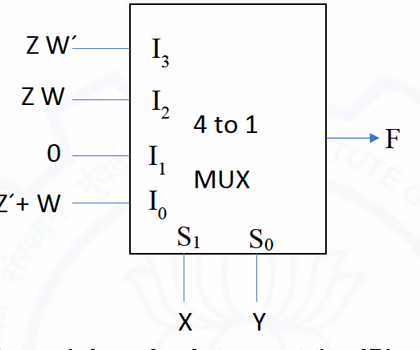
\includegraphics[width=0.5\linewidth]{Figs/Q-35.png}
    \caption{Multiplexer}
    \label{35}
\end{figure}

\begin{enumerate}[label=(\Alph*)]
\begin{multicols}{2}
\item $F\brak{X,Y,Z,W} = \Sigma m\brak{0,1,3,14,15}$
\item $F\brak{X,Y,Z,W} = \Sigma m\brak{0,1,3,11,14}$
\item $F\brak{X,Y,Z,W} = \Sigma m\brak{2,5,9,11,14}$
\item $F\brak{X,Y,Z,W} = \Sigma m\brak{1,3,7,9,15}$
\end{multicols}
\end{enumerate}

% Q.36
\item Given below in \figref{36} is the diagram of a synchronous sequential circuit with one J-K flip-flop and one T flip-flop with their outputs denoted as $A$ and $B$ respectively, with $J_A = \brak{A' + B'}$, $K_A = \brak{A + B}$, and $T_B = A$. Starting from the initial state ($AB=00$), the sequence of states ($AB$) visited by the circuit is
\begin{figure}[H]
    \centering
    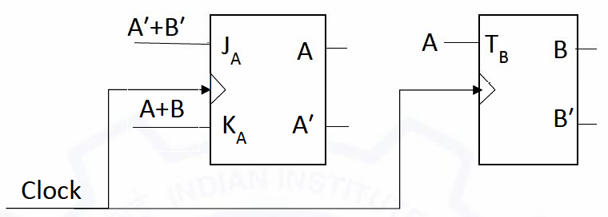
\includegraphics[width=0.5\linewidth]{Figs/Q-36.png}
    \caption{Synchronous Sequential Circuit}
    \label{36}
\end{figure}\par \hfill\brak{\text{GATE IN 2021}}
\begin{enumerate}[label=(\Alph*)]
\item $00 \to 01 \to 10 \to 11 \to 00 \dots$
\item $00 \to 10 \to 01 \to 11 \to 00\dots$
\item $00 \to 10 \to 11 \to 01 \to 00\dots$
\item $00 \to 01 \to 11 \to 00\dots$
\end{enumerate}

% Q.37
\item Consider that $X$ and $Y$ are independent continuous valued random variables with uniform PDF given by $X \sim U\brak{2,3}$ and $Y \sim U\brak{1,4}$. Then $P\brak{Y \le X}$ is equal to \rule{1.5cm}{0.4pt} (rounded off to two decimal places). \par \hfill\brak{\text{GATE IN 2021}}

% Q.38
\item Given $A = \myvec{2&5 \\ 0&3}$.  
The value of the determinant $|A^4 -5A^3 +6A^2 +2I| =$ \rule{1.5cm}{0.4pt}. \par \hfill\brak{\text{GATE IN 2021}}

% Q.39
\item \figref{;;} shows an electrically conductive bar of square cross-section resting on a plane surface. The bar of mass of $1\ \text{kg}$ has a depth of $0.5\ \text{m}$ along the $y$ direction. The coefficient of friction between the bar and the surface is $0.1$. Assume the acceleration due to gravity to be $10\ \text{m/s}^2$. The system faces a
uniform flux density $B = -1\hat{z}\ \text{T}$. At time $t=0$, a current of $10\ \text{A}$ is switched onto the bar and is maintained.
\begin{figure}[H]
    \centering
    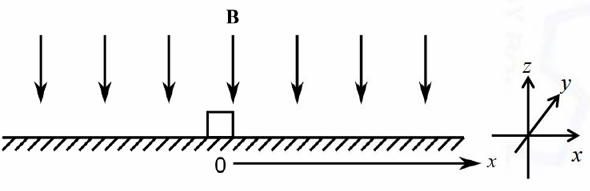
\includegraphics[width=0.5\linewidth]{Figs/Q-39.png}
    \caption{Electrically Conductive Bar resting on a plane surface}
    \label{;;}
\end{figure}
When the bar has moved by $1\ \text{m}$, its speed in metre per second is
\rule{1.5cm}{0.4pt} (rounded off to one decimal place). \par \hfill\brak{\text{GATE IN 2021}}

% Q.40
\item A toroid made of CRGO has an inner diameter of $10\ \text{cm}$ and an outer diameter of $14\ \text{cm}$. The thickness of the toroid is $2\ \text{cm}$. $200$ turns of copper wire is wound on the core. $\mu_0 = 4\pi\times10^{-7}\ \text{H/m}$ and $\mu_r$ of CRGO is $3000$. When
a current of $5\ \text{mA}$ flows through the winding, the flux density in the core in millitesla is \rule{1.5cm}{0.4pt}. \par \hfill\brak{\text{GATE IN 2021}}

% Q.41
\item An air cored coil having a winding resistance of $10\ \ohm$ is connected in series with a variable capacitor $C_x$. The series circuit is excited by a $10\ \text{V}$ sinusoidal voltage source of angular frequency $1000\ \text{rad/s}$. As the value of the capacitor
is varied, a maximum voltage of $30\ \text{V}$ was observed across it. Neglecting skin-effect, the value of the inductance of the coil in millihenry is \rule{1.5cm}{0.4pt}. \par \hfill\brak{\text{GATE IN 2021}}

% Q.42
\item A household fan consumes $60\ \text{W}$ and draws a current of $0.3125\ \text{A}$ (rms) when connected to a $230\ \text{V}$ (rms), $50\ \text{Hz}$ single phase mains. The reactive power drawn by the fan in $\text{VAr}$ is \rule{1.5cm}{0.4pt} (rounded off to the nearest integer). \par \hfill\brak{\text{GATE IN 2021}}

% Q.43
\item Given $y\brak{t} = e^{-3t}u\brak{t} * u\brak{t + 3}$, where $*$ denotes convolution operation. The value of $y\brak{t}$ as $t \to \infty$ is \rule{1.5cm}{0.4pt} (rounded off to two decimal places). \par \hfill\brak{\text{GATE IN 2021}}

% Q.44
\item The input signal shown in \figref{fig:placeholder_44(1)}
\begin{figure}[H]
    \centering
    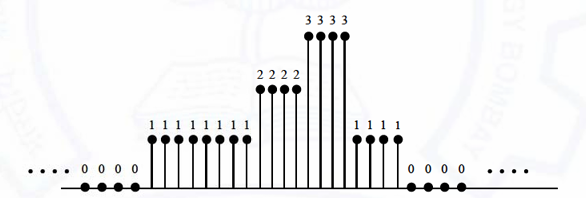
\includegraphics[width=0.6\linewidth]{Figs/Q-44(fig-1).png}
    \caption{Input Signal}
    \label{fig:placeholder_44(1)}
\end{figure}is passed through the filter with the following taps (\figref{fig:placeholder_44(2)})
\begin{figure}[H]
    \centering
    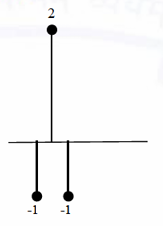
\includegraphics[width=0.2\linewidth]{Figs/Q-44(fig-2).png}
    \caption{Taps}
    \label{fig:placeholder_44(2)}
\end{figure}  
The number of non-zero output samples is \rule{1.5cm}{0.4pt}. \par \hfill\brak{\text{GATE IN 2021}}

% Q.45
\item A sinusoid $\brak{\sqrt{2}\sin t}\mu\brak{t}$, where $\mu\brak{t}$ is the step input, is applied to a system with transfer-function $G\brak{s} = \frac{1}{s+1}$. The amplitude of the steady state output is \rule{1.5cm}{0.4pt}. \par \hfill\brak{\text{GATE IN 2021}}

% Q.46
\item Consider a system with transfer-function $G\brak{s} = \dfrac{2}{s+1}$. A unit step function
$u\brak{t}$ is applied to the system, which results in an output $y\brak{t}$.
If $e\brak{t} = y\brak{t} - u\brak{t}$, then $\lim_{t \to \infty} e\brak{t} =$ \rule{1.5cm}{0.4pt}. \par \hfill\brak{\text{GATE IN 2021}}

% Q.47
\item The circuit shown in \figref{47} uses an ideal OpAmp. Output $V_o$ in volt is \rule{1.5cm}{0.4pt} (rounded off to one decimal place). \par \hfill\brak{\text{GATE IN 2021}}
\begin{figure}[H]
    \centering
    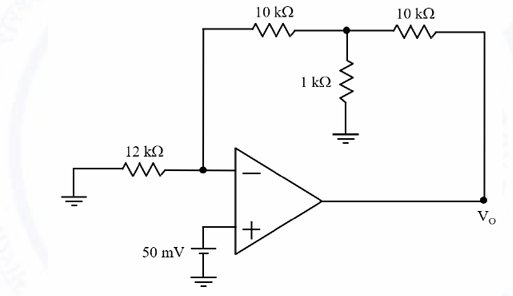
\includegraphics[width=0.5\linewidth]{Figs/Q-47.png}
    \caption{Caption}
    \label{47}
\end{figure}

% Q.48
\item All the transistors used in the circuit(\figref{48}) are matched and have a current gain $\beta$ of $20$. Neglecting the Early effect, the current $I_{04}$ in milliampere is \rule{1.5cm}{0.4pt}. \par \hfill\brak{\text{GATE IN 2021}}
\begin{figure}[H]
    \centering
    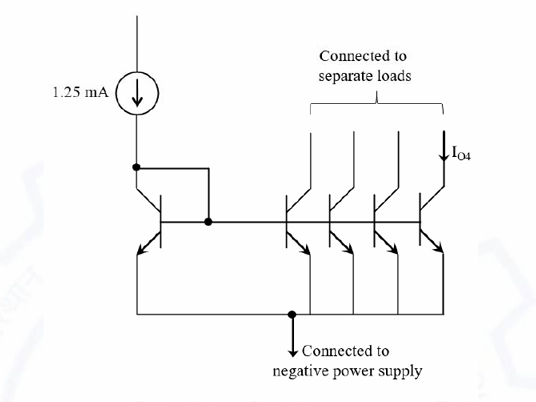
\includegraphics[width=0.5\linewidth]{Figs/Q-48.png}
    \caption{Caption}
    \label{48}
\end{figure}

% Q.49
\item The power in a $400\ \text{V}$ (rms, line-line) three-phase, three-wire RYB sequence system is measured using the two wattmeters, as shown in \figref{49}. The R-line current is $5\angle 60^\degree\ \text{A}$. Wattmeter $W_1$ in the R-line will read (in watt) \rule{1.5cm}{0.4pt}. \par \hfill\brak{\text{GATE IN 2021}}
\begin{figure}[H]
    \centering
    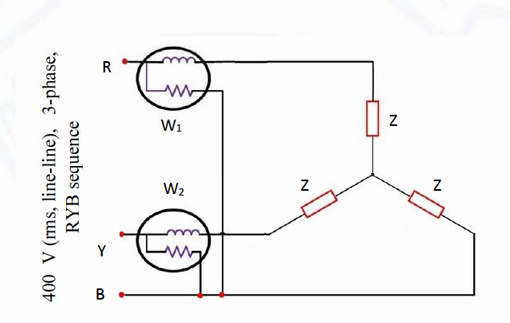
\includegraphics[width=0.5\linewidth]{Figs/Q-49.png}
    \caption{Caption}
    \label{49}
\end{figure}

% Q.50
\item A $3\frac{1}{2}$ digit, rectifier type digital meter is set to read in its $2000\ \text{V}$ range. A symmetrical square wave of frequency $50\ \text{Hz}$ and amplitude $\pm 100\ \text{V}$ is measured using the meter. The meter will read \rule{1.5cm}{0.4pt}. \par \hfill\brak{\text{GATE IN 2021}}

% Q.51
\item A bar primary current transformer of rating $1000/1\ \text{A}$, $5\ \text{VA}$, UPF has $995$ secondary turns. It exhibits zero ratio error and phase error of $30$ minutes at $1000\ \text{A}$ with rated burden. The watt loss component of the primary excitation current in ampere is \rule{1.5cm}{0.4pt} (rounded off to one decimal place). \par \hfill\brak{\text{GATE IN 2021}}

% Q.52
\item In the bridge circuit shown in \figref{52}, the voltmeter V showed zero when the value of the resistors are: $R_1 = 100\ \ohm$, $R_2 = 110\ \\ohm$, $R_3 = 90\ \\ohm$. If $\frac{R_1}{R_2} = \frac{R_A}{R_B}$,
the value of $R_4$ in ohm is \rule{1.5cm}{0.4pt}. \par \hfill\brak{\text{GATE IN 2021}}
\begin{figure}[H]
    \centering
    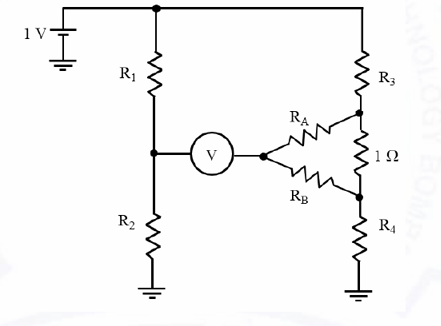
\includegraphics[width=0.5\linewidth]{Figs/Q-52.png}
    \caption{Caption}
    \label{52}
\end{figure}

% Q.53
\item For the full bridge made of linear strain gages with gage factor $2$ as shown in \figref{53}, $R1 = R2 = R3 = R4 = 100\ohm$ at $0^\degree\text{C}$ and strain is $0$. The temperature coefficient of resistance of the strain gages used is $0.005$ per $^\degree \text{C}$.
All strain gages are made of same material and exposed to same
temperature. While measuring a strain of $0.01$ at a temperature of $50^\circ \text{C}$, the
output $V_o$ in millivolt is \rule{1.5cm}{0.4pt} (rounded off to two decimal places). \par \hfill\brak{\text{GATE IN 2021}}
\begin{figure}[H]
    \centering
    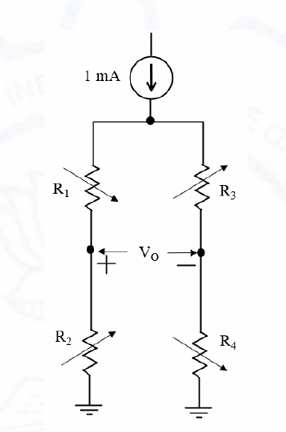
\includegraphics[width=0.3\linewidth]{Figs/Q-53.png}
    \caption{Caption}
    \label{53}
\end{figure}

% Q.54
\item A signal having a bandwidth of $5\ \text{MHz}$ is transmitted using the Pulse code modulation (PCM) scheme as follows. The signal is sampled at a rate of $50\ \%$ above the Nyquist rate and quantized into $256$ levels. The binary pulse rate of the PCM signal in Mbits per second is \rule{1.5cm}{0.4pt}. \par \hfill\brak{\text{GATE IN 2021}}

% Q.55
\item In \figref{55}, a large multimode fiber with $n_{core} = 1.5$ and $n_{clad} =1.2$ is used for sensing. A portion with the cladding removed passes through a liquid with refractive index $n_{liquid}$. An LED is used to illuminate the fiber from one end and a paper is placed on the other end, $1\ \text{cm}$ from the end of the fiber. The paper shows a spot with radius $1\ \text{cm}$. The refractive index $n_{liquid}$ of the liquid (rounded off to two decimal places) is \rule{1.5cm}{0.4pt}. \par \hfill\brak{\text{GATE IN 2021}}
\begin{figure}[H]
    \centering
    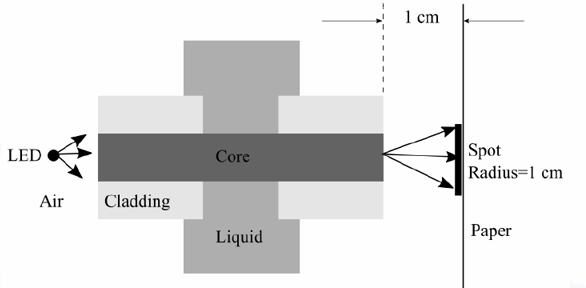
\includegraphics[width=0.5\linewidth]{Figs/Q-55.png}
    \caption{Caption}
    \label{55}
\end{figure}

\end{enumerate}

\end{document}

